\documentclass[runningheads]{llncs}
\usepackage[utf8]{inputenc}
\usepackage{amsmath}
\usepackage{amssymb}
\usepackage{tikz}
\usetikzlibrary{backgrounds}
\usepackage{tikz-qtree}
\usetikzlibrary{shapes, arrows}

\begin{document}

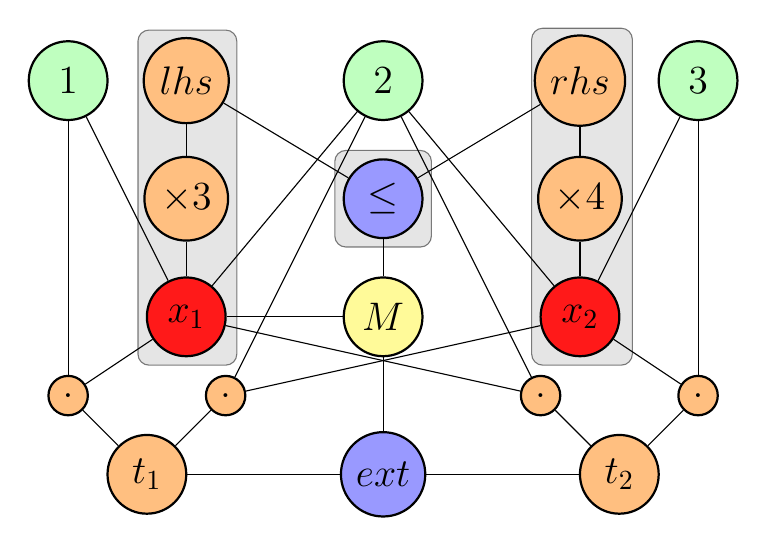
\begin{tikzpicture}[>=stealth',auto,node distance=2.0cm,
  thick,main node/.style={circle,fill=blue!20,draw,
  font=\sffamily\Large\bfseries,minimum size=10mm}]
  \pgfdeclarelayer{background}
  \pgfsetlayers{background,main}


  \node[main node, fill=green!25] (value_1) at (-4, 2) {$1$};
  \node[main node, fill=green!25] (value_2) at (-0, 2) {$2$};
  \node[main node, fill=green!25] (value_3) at (4, 2) {$3$};

  \node[main node, fill=red!90] (x_1) at (-2.5,-1) {$x_1$};
  \node[main node, fill=red!90] (x_2) at (2.5,-1) {$x_2$};

  \node[main node, fill=orange!50] (mul_1) at (-2.5, 0.5) {$\times 3$};
  \node[main node, fill=orange!50] (mul_2) at (2.5, 0.5) {$\times 4$};

  \node[main node, fill=orange!50] (lhs) at (-2.5, 2) {$lhs$};
  \node[main node, fill=orange!50] (rhs) at (2.5, 2) {$rhs$};

  \node[main node, fill=blue!40] (leq) at (0,0.5) {$\leq$};

  \node[main node, fill=orange!50] (tup1) at (-3,-3)  {$t_1$};
  \node[main node, fill=orange!50] (tup2) at (3,-3)  {$t_2$};

  \node[main node, fill=orange!50, minimum size=5mm] (combo11) at (-4,-2)  {$.$};
  \node[main node, fill=orange!50, minimum size=5mm] (combo22) at (-2,-2)  {$.$};

  \node[main node, fill=orange!50, minimum size=5mm] (combo21) at (2,-2)  {$.$};
  \node[main node, fill=orange!50, minimum size=5mm] (combo23) at (4, -2)  {$.$};

  \node[main node, fill=blue!40] (ext) at (0,-3) {$ext$};
  \node[main node, fill=yellow!40] (model) at (0,-1) {$M$};
  \begin{pgfonlayer}{background}
    \draw[rounded corners, fill=gray!40, opacity=0.5] 
        ([shift={(-0.25cm,-0.25cm)}]x_1.south west) rectangle 
        ([shift={(0.25cm,0.25cm)}]lhs.north east);
    \draw[rounded corners, fill=gray!40, opacity=0.5] 
        ([shift={(-0.25cm,-0.25cm)}]x_2.south west) rectangle 
        ([shift={(0.25cm,0.25cm)}]rhs.north east);
    \draw[rounded corners, fill=gray!40, opacity=0.5] 
        ([shift={(-0.25cm,-0.25cm)}]leq.south west) rectangle 
        ([shift={(0.25cm,0.25cm)}]leq.north east);
  \end{pgfonlayer}

  \path[every node/.style={font=\sffamily\small, fill=white,}]
    (x_1) edge[black] (value_1)
    (x_1) edge[black] (value_2)
    (x_1) edge[black] (mul_1)
    (mul_1) edge[black] (lhs)
    (rhs) edge[black] (leq)

    (x_2) edge[black] (value_2)
    (x_2) edge[black] (value_3)
    (x_2) edge[black] (mul_2)
    (mul_2) edge[black] (rhs)
    (lhs) edge[black] (leq)

    % Black edges between variables and tuples
    (x_1) edge[black] (combo21)
    (x_1) edge[black] (combo11)

    (x_2) edge[black] (combo22)
    (x_2) edge[black] (combo23)

    % Black edges between values and tuples
    (value_1) edge[black] (combo11)
    (value_2) edge[black] (combo22)
    (value_2) edge[black] (combo21)
    (value_3) edge[black] (combo23)

    (tup1) edge[black] (combo11)
    (tup1) edge[black] (combo22)

    (tup2) edge[black] (combo21)
    (tup2) edge[black] (combo23)

    (tup1) edge[black] (ext)
    (tup2) edge[black] (ext)

    (model) edge[black] (ext)
    (model) edge[black] (leq)
    (model) edge[black] (x_1)
    ;
\end{tikzpicture}

\end{document}